% Created 2020-10-31 六 00:29
% Intended LaTeX compiler: xelatex
\documentclass[11pt]{report}
\usepackage{graphicx}
\usepackage{grffile}
\usepackage{longtable}
\usepackage{wrapfig}
\usepackage{rotating}
\usepackage[normalem]{ulem}
\usepackage{amsmath}
\usepackage{textcomp}
\usepackage{amssymb}
\usepackage{capt-of}
\usepackage{hyperref}
\author{曹嘉祺 PB18030874 化学与材料科学学院 有机化学系 \thanks{中国 安徽合肥 中国科学技术大学 Email: \href{mailto:mkq@mail.ustc.edu.cn}{mkq@mail.ustc.edu.cn}}}
\usepackage[scheme=plain]{ctex}
\usepackage{fontspec}
\setmainfont{新蒂下午茶体}
\hypersetup{colorlinks=true,linkcolor=blue}
\usepackage{longtable}
\date{\today}
\title{溶液中的吸附作用和表面张力的测定\\\medskip
\large 最大气泡压力法}
\hypersetup{
 pdfauthor={曹嘉祺 PB18030874 化学与材料科学学院 有机化学系},
 pdftitle={溶液中的吸附作用和表面张力的测定},
 pdfkeywords={表面张力 表面能 吸附作用 表面活性物质 Langmuir等温方程式 最大气泡法 饱和吸附量},
 pdfsubject={},
 pdfcreator={Emacs 27.1 (Org mode 9.4)}, 
 pdflang={English}}
\begin{document}

\maketitle
\begin{abstract}
本实验通过了解表面张力的性质、表面能的意义以及表面张力和吸附的关系,
并学习最大气泡法测表面张力的原理和方法。用最大气泡法测定不同浓度正丁醇水溶液的表
面张力\(\sigma\),并利用它来研究溶液中的吸附作用。作\(\sigma\)-c 曲线并求曲线在不同浓度下的斜率
来求溶液界面上的吸附量。进而作\(\frac{c}{\Gamma}-c\) 曲线,由直线斜率求出饱和吸附量 \(\Gamma\)\textsubscript{\(\infty\)} ,
并根据公式:
\[
S_{0}=\frac{1}{\Gamma_{\infty}\widetilde{N}}
\]
由 \(\Gamma\)\textsubscript{\(\infty\)} 计算单个正丁醇分子的横截面积(S\textsubscript{0}) 。

\noindent\rule{\textwidth}{0.5pt}
\begin{itemize}
\item 关键词: 表面张力\quad 表面能\quad 吸附作用\quad 表面活性物质\quad Langmuir等温方程式\quad 最大气泡法\quad 饱和吸附量
\end{itemize}
\end{abstract}




\begin{abstract}



In this experiment, we learn the knowledge of surface tension, surface energy and
maximum bubble method. Then we use maximum bubble method to measure the surface tension
of n-butyl alcohol at different concentration, and we can use the data to study adsorption in
solution. And we can use of the Gibbs formula:
\[
\Gamma = −\frac{c}{RT}\left(\frac{\partial \sigma}{\partial c}\right)_{T}
\]
and Langmuir isothermal equation:
\[
\frac{C}{\Gamma}=\frac{C}{\Gamma_{\infty}}+\frac{1}{KT_{\infty}}
\]
 etc. to study the relations between the concentration of the solution
and surface tension as well as the amount of absorption, finally we can calculate the cross
sectional area of n-butyl alcohol.

\noindent\rule{\textwidth}{0.5pt}

\begin{itemize}
\item key words: surface tension, surface energy, adsorption, surface active agent, Langmuir isothermal equation, maximum bubble method, n-butyl alcohol
\end{itemize}
\end{abstract}
\part{前言}
\label{sec:org396f0df}
\chapter{表面张力及表面能的概念}
\label{sec:org7945991}
物体表面的分子和内部分子所处的境况不同,因而能量也不同,表面层的
分子受到向内的拉力,所以液体表面都有自动缩小的趋势.如要把一个分子由内部迁移到表
面,就需要对抗拉力而作功,故表面分子的能量比内部分子大。增加体系的表面,即增加了
体系的总能量。体系产生新的表面(\(\Delta\) A)所需耗费功(W)的量,其大小应与\(\Delta\) A 成正比。
\[
-W=\sigma \Delta A
\]
如果\(\Delta\) A=1m\textsuperscript{2},则-W=\(\sigma\),即在等温下形成 1m\textsuperscript{2}
新的表面所需的可逆功。故\(\sigma\) 称为单位表面的表面能,
其单位为 N\(\cdot\) m\textsuperscript{-1}。这样就把\(\sigma\) 看作为作用在界面上每单位长度边缘上的力,
通常称为表面张力。它表示表面自动缩小的趋势的大小。表面张力是液体的重要特性之一,
与所处的温度、压力、液体的组成共存的另一相的组成等有关。纯液体的表面张力通常指该
液体与饱和了其自身蒸气的空气共存的情况而言。
\chapter{表面张力与吸附作用及表面活性物质}
\label{sec:org8319af2}
在纯液体情形下,表面层的组成与内部的组成相同, 因此液体降低体系表面自由能的唯
一途径是尽可能缩小其表面积。对于溶液,由于溶质会影响表面张力,因此可以调节溶质在
表面层的浓度来降低表面自由能。
根据能量最低原理,溶质能降低溶液的表面张力时,表面层中溶质的浓度应比溶液内部
大,反之,溶质使溶液的表面张力升高时,它在表面层中的浓度比在内部的浓度低。这种表
面浓度与溶液里面浓度不同的现象叫“吸附”。显然,在指定温度和压力下,吸附与溶液的
表面张力及溶液的浓度有关。Gibbs 用热力学的方法推导出它们间的关系式:
\[
\Gamma = - \frac{c}{RT}	\left(\frac{\partial \sigma}{\partial c}\right)_{T}
\]

\begin{itemize}
\item \(\Gamma\):气一液界面上的吸附量(mol·m\textsuperscript{-2});
\item \(\sigma\):溶液的表面张力(N·m\textsuperscript{-1});
\item T:绝对温度(K)
\item c:溶液浓度(mol·m\textsuperscript{-3});
\item R:气体常数(8.314J\(\cdot\) mol\textsuperscript{-1}\(\cdot\) K\textsuperscript{-1})。
\end{itemize}

当\(\left(\frac{\partial \sigma}{\partial c}\right)_{T}<0\) 时,\(\Gamma\)>0,称为正吸附.
反之,\(\left(\frac{\partial \sigma}{\partial c}\right)_{T}<0\) 时,\(\Gamma\)<0,称为负吸附.
前者表明加入溶质使液体表面张力下降, 此类物质叫表面活性物质, 后者表明加入溶质使液体表面
张力升高,此类物质叫非表面活性物质。

表面活性物质具有显著的不对称结构,它是由亲水的极性部分和憎水的非极性部分构
成。 对于有机化合物来说,表面活性物质的极性部分一般为-NH\textsubscript{3}\textsuperscript{+},-OH,-SH,-COOH,
-SO\textsubscript{2}OH。而非极性部分则为 RCH\textsubscript{2}-。正丁醇就是这样
的分子。在水溶液表面的表面活性物质分子,其极性部分
朝向溶液内部,而非极性部分朝向空气。表面活性物质分
子在溶液表面的排列情形随其在溶液中的浓度不同而有
所差异。当浓度极小时,溶质分子平躺在溶液表面上,
当浓度增加到一定程度时,被吸附了的表面活性物质
分子占据了所有表面形成了单分子的饱和吸附层.

正丁醇是一种表面活性物质,其水溶液的表面张力和
浓度关系见图 11-3 中的\(\sigma\)-c 曲线,在\(\sigma\)-c 曲线上作不
同浓度 c 时的切线,把切线的斜率\(B\left(\left(\frac{\partial \sigma}{\partial c}\right)_{T}\right)\)
代入Gibbs吸附公式,可以求出不同浓度时气-液界面上的吸附量\(\Gamma\)。

在一定温度下,吸附量与溶液浓度之间的关系由 Langmuir 等温方程式表示:
\[
\Gamma=\Gamma_{\infty}\frac{K\cdot C}{1+K\cdot C}
\]
\(\Gamma\)\textsubscript{\(\infty\)}为饱和和吸附量,K 为经验常数,与溶质的表面活性大小有关。将上式化成直线方程,有:
\[
\frac{C}{\Gamma}=\frac{C}{\Gamma_{\infty}}+\frac{1}{KT_{\infty}}
\]

若以\(\frac{C}{\Gamma}-C\) 作图可得一直线,由直线斜率即可求出\(\Gamma\)\textsubscript{\(\infty\)} 。

假设在饱和吸附情况下,正丁醇分子在气-液界面上铺满一单分子层,则可应用下式求得正丁醇分子的横截面积 S\textsubscript{0}.
\[
S_{0}=\frac{1}{\Gamma_{\infty}\widetilde{N}}
\]
\begin{itemize}
\item \widetilde{N}: 阿伏加德罗常数
\end{itemize}


\chapter{最大气泡法测量表面张力的原理及方法}
\label{sec:org5571713}
最大气泡压力法测量表面张力的装置示意图如2
11-4。当,表面张力仪中的毛细管截面与欲测液面相齐时,液面沿毛细管上升。打开滴液漏斗的活塞,
使水缓慢下滴而使体系内的压力增加, 这时毛细管内的液面上受到一个比恒温试管中液面上
稍大的压力, 因此毛细管内的液面缓缓下降。 当此压力差在毛细管端面上产生的作用力稍大
于毛细管口溶液的表面张力时,气泡就从毛细管口逸出。 这个最大的压力差可由数字式微压
差测量仪上读出。

如毛细管的半径为 r,气泡由毛细管口逸出时受到向下的总作用力为 \(\pi\) r\textsuperscript{2}P\textsubscript{max}, 则有:
\[
P_{max}=P_{system}-P_{0}=\Delta h\rho g
\]
\begin{itemize}
\item \(\Delta\) h:数字式微压差测量仪上的读数
\item g:重力加速度
\item \(\rho\):压力计内液体的密度
\end{itemize}
气泡在毛细管上受到表面张力引起的作用力为 2\(\pi\) r\(\sigma\) 。气泡自毛细管口逸出时,上述两种力
看作相等,即:
\[
\pi r^{2}P_{max}=\pi r^{2}\Delta h\rho g
\]
\[
\sigma=\frac{r}{2}\Delta h\rho g
\]

若用同一只毛细管和压力计,在同一温度下,对两种溶液而言,则得:
\[
\frac{\sigma_{1}}{\sigma_{2}}=\frac{\Delta h_{1}}{\Delta h_{2}}
\]
\[
\sigma_{1}=\frac{\sigma_{2}}{\Delta h_{2}}\Delta h_{1}=K'\Delta h_{1}
\]
式中 K' 为毛细管常数。

用已知表面张力\(\sigma\)\textsubscript{2} 的液体为标准,从上式可求出其他液体的表面张力\(\sigma\)\textsubscript{1}。




\part{实验部分}
\label{sec:org648ea67}
\chapter{实验过程}
\label{sec:org273cbdb}
\section{实验仪器与试剂}
\label{sec:orgcc19e9d}
\begin{center}
\begin{tabular}{llll}
仪器 & 数目 & 仪器 & 数目\\
\hline
超级恒温水浴 & 1台 & 数字式微压差测量仪 & 1台\\
恒温套管 & 1支 & 毛细管(半径为 0.15\textasciitilde{}0.2mm) & 1支\\
100mL 容量瓶 & 7个 & 2mL 移液管 & 1支\\
250mL 分液漏斗 & 1个 & 500mL 塑料烧杯 & 1个\\
正丁醇(分析纯) &  &  & \\
\end{tabular}
\end{center}
\section{实验步骤}
\label{sec:org1d04df5}
\begin{enumerate}
\item 配制不同浓度的正丁醇溶液
\label{sec:orgc484ddd}
用 2mL 移液管分别移取 0.40ml、0.80ml、1.20ml、1.60ml、2.00ml、2.40ml、2.80ml 正
丁醇到 100ml 容量瓶中,稀释定容,置于 25°C恒温水浴中恒温备用。
\item 测定纯水的表面张力,记录压力差\(\Delta\) p,并由此确定毛细管常数
\label{sec:org65153d6}
取一支浸泡在洗液中的毛细管依次次用丙酮、 蒸馏水反复清洗若干次,同样把玻璃套管
也清洗干净,加上蒸馏水,插上毛细管,用套管下端的开关调节液面恰好与毛细管端面相切
(相切较难把握,需仔细判断),使样品在其中恒温 10 分钟。本实验采用机器控制使水慢
慢滴下,这时体系压力逐渐减小,直至气泡由毛细管口冒出,细心调节机器转速,使出泡
速度在 5-10 秒钟内出一个较好。 注意气泡爆破前数字式微压差测量仪的读数,并用电脑采
集数据得到最大的压差值,求平均值而得 \(\Delta\) p\textsubscript{H\textsubscript{2}O} 。根据手册查出 25°C时水的表面张力为
\(\sigma\)=71.97\texttimes{} 10\textsuperscript{-3}N\(\cdot\) m\textsuperscript{-1},以\(\sigma\)/\(\Delta\) p=K 求出所使用的毛细管常数,
此值控制在 8cm 左右为宜,否则
毛细管太粗误差较大,毛细管太细,易堵塞,气泡很难逸出。
\item 测定不同浓度正丁醇的表面张力
\label{sec:orgc8f452b}
将毛细管和内的残余液体用吸耳球吹尽,毛细管外壁用下一个待测液冲洗干净,将玻
璃管用待测液润洗两次, 再将上述配制好的正丁醇溶液按照由稀至浓的顺序依次加入玻璃管
中,重复上述步骤进行测量。
 (每次测量前都要进行洗涤及润洗工作)
\item 注意事项:
\label{sec:org233f4a4}
\begin{itemize}
\item 测定用的毛细管一定要先洗干净,否则气泡可能不能连续稳定地通过,而使压力计的读数不稳定。
\item 毛细管一定要垂直,管口要和液面刚好接触。
\item 表面张力和温度有关,因此要等溶液恒温后再测量。
\item 控制好出泡速度,读取压力计的压力差时,应取气泡单个逸出时的最大压力差。
\end{itemize}
\end{enumerate}

\chapter{实验结果与讨论}
\label{sec:orgaf3b164}
\section{实验数据及处理结果}
\label{sec:orgad339a6}

\begin{enumerate}
\item 纯水表面张力及毛细管常数的计算
\label{sec:orga9e4dd1}
     由 25°C时水的表面张力为 \(\sigma\)=71.97\texttimes{} 10\textsuperscript{-3}N\(\cdot\) m\textsuperscript{-1} 可知:
毛细管常数 K 为:K=\(\sigma\)/\(\Delta\) p=71.97/562=2.2703\texttimes{} 10\textsuperscript{-4}(m)
\item 不同浓度正丁醇溶液的表面张力的计算:
\label{sec:orgfda1f74}
\begin{enumerate}
\item 0.8mL 正丁醇
\label{sec:orgf716a79}
正丁醇浓度为:0.8\texttimes{} 0.8109/(74.14\texttimes{} 0.1)=0.08750 mol/L=87.50 mol/m\textsuperscript{3}.
表面张力为:
\[
    \sigma=K\cdot \Delta p=2.2703\times 10^{-4}\times 273=61.98\times 10^{-3}(N\cdot m^{-1})
    \]

\item 1.2mL 正丁醇
\label{sec:org04d5916}
正丁醇浓度为:1.2\texttimes{} 0.8109/(74.14\texttimes{} 0.1)=0.13125 mol/L=131.25 mol/m\textsuperscript{3}.

可得表面张力为:
\[
    \sigma=K\cdot \Delta p=2.2703\times 10^{-4}\times 246=55.85\times 10^{-3}(N\cdot m^{-1})
    \]

\item 1.6mL 正丁醇
\label{sec:orgcfc1c2e}
正丁醇浓度为:1.6\texttimes{} 0.8109/(74.14\texttimes{} 0.1)=0.17500 mol/L=175.00 mol/m\textsuperscript{3}.

表面张力为:
\[
    \sigma=K\cdot \Delta p=2.2703\times 10^{-4}\times 238=54.03\times 10^{-3}(N\cdot m^{-1})
    \]

\item 2.0mL 正丁醇
\label{sec:org19fccea}
正丁醇浓度为:2.0\texttimes{} 0.8109/(74.14\texttimes{} 0.1)=0.21875 mol/L=218.75 mol/m\textsuperscript{3}.

可得表面张力为:
\[
    \sigma=K\cdot \Delta p=2.2703\times 10^{-4}\times 232=52.67\times 10^{-3}(N\cdot m^{-1})
    \]

\item 2.4mL 正丁醇
\label{sec:org984724a}
正丁醇浓度为:2.4\texttimes{} 0.8109/(74.14\texttimes{} 0.1)=0.26250 mol/L=262.50 mol/m\textsuperscript{3}.

可得表面张力为:
\[
    \sigma=K\cdot \Delta p=2.2703\times 10^{-4}\times 224=50.85\times 10^{-3}(N\cdot m^{-1})
    \]

\item 2.8mL 正丁醇
\label{sec:org8b0a375}
正丁醇浓度为:2.8\texttimes{} 0.8109/(74.14\texttimes{} 0.1)=0.30625 mol/L=306.25 mol/m\textsuperscript{3}.

可得表面张力为:
\[
    \sigma=K\cdot \Delta p=2.2703\times 10^{-4}\times 211=47.90\times 10^{-3}(N\cdot m^{-1})
    \]
\end{enumerate}

\item 作表面张力与浓度(\(\sigma\)-c)的关系图,并求吸附量\(\Gamma\)
\label{sec:org7a70388}
根据公式:
\[
\Gamma=-\frac{c}{RT}\left(\frac{d\sigma}{dc}\right)
\]
\begin{center}
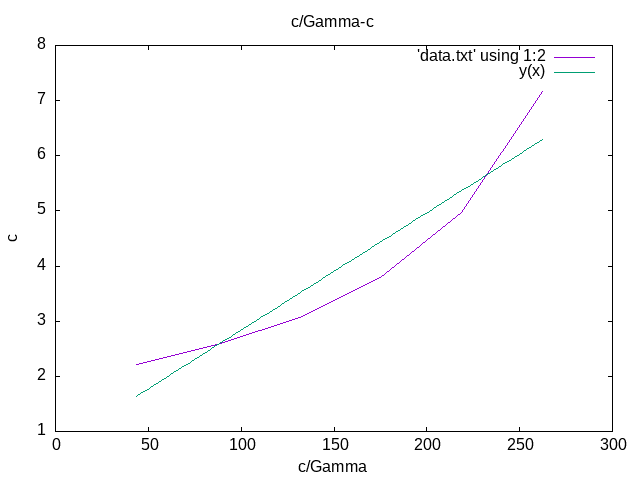
\includegraphics[width=.9\linewidth]{../img/out.png}
\end{center}
则
   \[
   \Gamma_{\infty}=\frac{1}{k}=4.699248\times 10^{-6} mol/m^{3}
   \]
   正丁醇分子的横截面积为:
   \[
   S_{0}=\frac{1}{\Gamma_{\infty}\widetilde{N}}=3.533627\times 10^{-19} m^{2}
   \]
\end{enumerate}

\section{结果分析与讨论}
\label{sec:orgc9e26a2}
\begin{enumerate}
\item 实验中在测量水及正丁醇的最大压差时,每次测完一组数据都要用丙酮、蒸馏水反复洗
涤毛细管,很费时,后经老师指导,若毛细管可正常出气泡,则可不必每次都经这么麻烦的
步骤去洗涤,可按下述步骤进行快速洗涤:将毛细管和内的残余液体用吸耳球吹尽,毛细
管外壁用下一个待测液冲洗干净,将玻璃管用待测液润洗两次。这么节省了不少时间,最
后测量结果也较好,但是最终在计算 \(\Gamma\)\textsubscript{\(\infty\)} ,所作的曲线线性不好,有可能就是这一步没洗干
净造成的。

\item 在进行多项式拟合时,曾经考虑用较高次的多项式进行拟合,但最后所得结果都无法较
好的反应曲线的趋势, 只有二次拟合所得曲线与数据走向趋势符合的很好, 虽然用高阶的多
项式可能所得拟合曲线的相关性较好, 但是由计算方法课中所学知识可知, 相关性的提高是
计算方法原理本身所决定的,并不能说明曲线与数据走向符合的较好, 所以最终选择了二次
多项式拟合,这样在数据处理时也较为方便,但是并不能保证一定是较好的方法,而且可能
带来一定误差。
\item 在计算吸附量时不同的拟合公式会对最后结果有较大影响,不同的公式会有不同的切线
方程,会得到不同的吸附量,而在计算 时,因为吸附量\Gamma在分母上,所以即使\Gamma有很小的
改变,对最后的计算结果仍有较大的影响,导致所作曲线不准确,最后所得的曲线线
性不好,可能与这也有一定的关系。
\end{enumerate}


\part{结论}
\label{sec:org525b459}
  本实验通过最大气泡法对水以及正丁醇最大压力差的测定,得出不同溶液表面张力的数值,
进而通过相关的数据处理, 得出正丁醇的饱和吸附量以及横截面积, 虽然最后的结果不是很
理想,但基本上在可接受的范围内,在低浓度下与理论也有较好的吻合。说明关于吸附的理
论在低浓度时较为准确,这也从另一方面证明了实验的合理性及准确性.
\part{参考文献}
\label{sec:org29752d7}
\begin{enumerate}
\item 中国科学技术大学化学实验教学中心物理化学实验讲义
\item 《物理化学下》傅献彩等编 高等教育出版社
\end{enumerate}

\part{附录: 数据处理过程}
\label{sec:org0d93497}
\chapter{纯水表面张力和毛细管常数的计算}
\label{sec:org1b6381e}
电脑记录数据做图如下:
\begin{center}
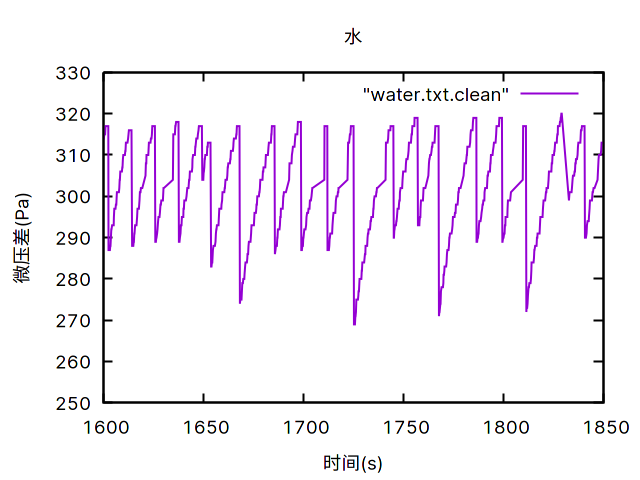
\includegraphics[width=.9\linewidth]{../img/water.png}
\end{center}
最大压强差读数数据记录如下:
\begin{center}
\begin{tabular}{lrrrrrrr}
序号 & 1 & 2 & 3 & 4 & 5 & 6 & 平均\\
\hline
最大压强差读数\(\Delta\) p(Pa) & 317 & 317 & 317 & 318 & 317 & 317 & 317\\
\end{tabular}
\end{center}


最大压强读数平均:
\[
    \Delta p =\frac{317\times 5 + 318}{6}=317(Pa)
    \]
由 25°C时水的表面张力为 \(\sigma\)=71.97\texttimes{} 10\textsuperscript{-3}N\(\cdot\) m\textsuperscript{-1} 可知
毛细管常数 K 为:
\[
    K=\sigma /\Delta p =71.97\times 10^{-3}/317=2.2703\times 10^{-4}(m)
    \]
\chapter{不同浓度正丁醇溶液的表面张力的计算}
\label{sec:org7c960de}

\section{0.4mL 正丁醇}
\label{sec:org2809f80}
    100 mL 容量瓶中含 0.4 mL 正丁醇。由于正丁醇分子量为 74.14,密度为 0.8109 g/cm\textsuperscript{3}
故得正丁醇浓度为:0.4\texttimes{} 0.8109/(74.14\texttimes{} 0.1)=0.04375 mol/L=43.75 mol/m\textsuperscript{3}.

电脑记录数据作图如下:
\begin{center}
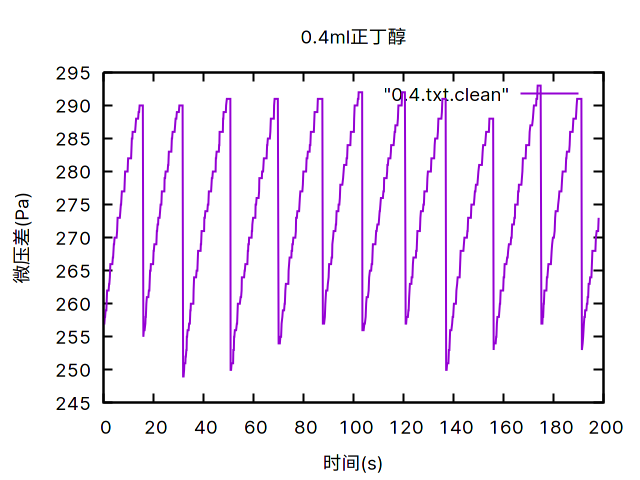
\includegraphics[width=.9\linewidth]{../img/0.4.png}
\end{center}

最大压强差读数数据记录如下:
\begin{center}
\begin{tabular}{lrrrrrrr}
序号 & 1 & 2 & 3 & 4 & 5 & 6 & 平均\\
\hline
最大压强差读数\(\Delta\) p(Pa) & 291 & 291 & 291 & 292 & 292 & 291 & 291\\
\end{tabular}
\end{center}


最大压强读数平均:
\[
    \Delta p =\frac{291\times 4 + 292 \times 2}{6}=291(Pa)
    \]
由公式 \(\sigma\)=K\(\cdot\) \(\Delta\) p 可得表面张力为:
\[
    \sigma=K\cdot \Delta p=2.2703\times 10^{-4}\times 291=66.07\times 10^{-3}(N\cdot m^{-1})
    \]

\section{0.8mL 正丁醇}
\label{sec:orgb751a0b}
    100 mL 容量瓶中含 0.8 mL 正丁醇。由于正丁醇分子量为 74.14,密度为 0.8109 g/cm\textsuperscript{3}
故得正丁醇浓度为:0.8\texttimes{} 0.8109/(74.14\texttimes{} 0.1)=0.08750 mol/L=87.50 mol/m\textsuperscript{3}.

电脑记录数据作图如下:
\begin{center}
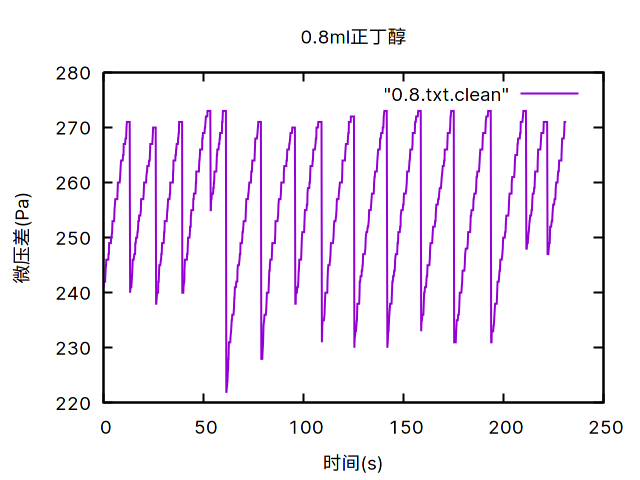
\includegraphics[width=.9\linewidth]{../img/0.8.png}
\end{center}

最大压强差读数数据记录如下:
\begin{center}
\begin{tabular}{lrrrrrrr}
序号 & 1 & 2 & 3 & 4 & 5 & 6 & 平均\\
\hline
最大压强差读数\(\Delta\) p(Pa) & 272 & 273 & 273 & 273 & 273 & 273 & 273\\
\end{tabular}
\end{center}

最大压强读数平均:
\[
    \Delta p =\frac{273\times 5 + 272}{6}=273(Pa)
    \]
由公式 \(\sigma\)=K\(\cdot\) \(\Delta\) p 可得表面张力为:
\[
    \sigma=K\cdot \Delta p=2.2703\times 10^{-4}\times 273=61.98\times 10^{-3}(N\cdot m^{-1})
    \]

\section{1.2mL 正丁醇}
\label{sec:orgd4cf7a9}
    100 mL 容量瓶中含 1.2 mL 正丁醇。由于正丁醇分子量为 74.14,密度为 0.8109 g/cm\textsuperscript{3}
故得正丁醇浓度为:1.2\texttimes{} 0.8109/(74.14\texttimes{} 0.1)=0.13125 mol/L=131.25 mol/m\textsuperscript{3}.

电脑记录数据作图如下:
\begin{center}
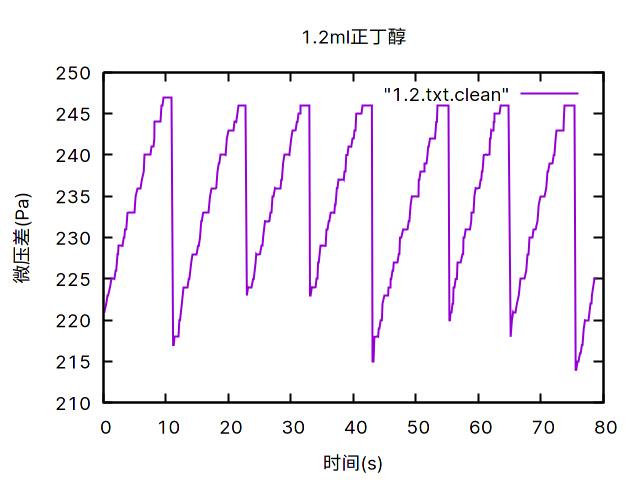
\includegraphics[width=.9\linewidth]{../img/1.2.png}
\end{center}

最大压强差读数数据记录如下:
\begin{center}
\begin{tabular}{lrrrrrrr}
序号 & 1 & 2 & 3 & 4 & 5 & 6 & 平均\\
\hline
最大压强差读数\(\Delta\) p(Pa) & 246 & 246 & 246 & 246 & 246 & 246 & 246\\
\end{tabular}
\end{center}

最大压强读数平均:
\[
    \Delta p =\frac{246\times 6}{6}=246(Pa)
    \]
由公式 \(\sigma\)=K\(\cdot\) \(\Delta\) p 可得表面张力为:
\[
    \sigma=K\cdot \Delta p=2.2703\times 10^{-4}\times 246=55.85\times 10^{-3}(N\cdot m^{-1})
    \]

\section{1.6mL 正丁醇}
\label{sec:org854dd1f}
    100 mL 容量瓶中含 1.6 mL 正丁醇。由于正丁醇分子量为 74.14,密度为 0.8109 g/cm\textsuperscript{3}
故得正丁醇浓度为:1.6\texttimes{} 0.8109/(74.14\texttimes{} 0.1)=0.17500 mol/L=175.00 mol/m\textsuperscript{3}.

电脑记录数据作图如下:
\begin{center}
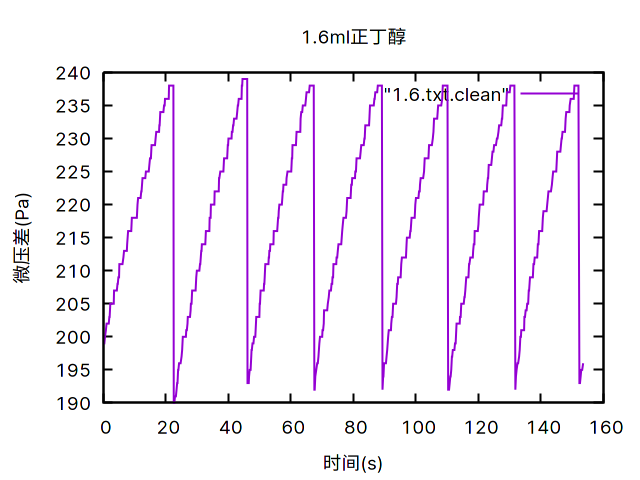
\includegraphics[width=.9\linewidth]{../img/1.6.png}
\end{center}

最大压强差读数数据记录如下:
\begin{center}
\begin{tabular}{lrrrrrrr}
序号 & 1 & 2 & 3 & 4 & 5 & 6 & 平均\\
\hline
最大压强差读数\(\Delta\) p(Pa) & 239 & 238 & 238 & 238 & 238 & 238 & 238\\
\end{tabular}
\end{center}

最大压强读数平均:
\[
    \Delta p =\frac{238\times 5+239}{6}=238(Pa)
    \]
由公式 \(\sigma\)=K\(\cdot\) \(\Delta\) p 可得表面张力为:
\[
    \sigma=K\cdot \Delta p=2.2703\times 10^{-4}\times 238=54.03\times 10^{-3}(N\cdot m^{-1})
    \]

\section{2.0mL 正丁醇}
\label{sec:org2732ca8}
    100 mL 容量瓶中含 2.0 mL 正丁醇。由于正丁醇分子量为 74.14,密度为 0.8109 g/cm\textsuperscript{3}
故得正丁醇浓度为:2.0\texttimes{} 0.8109/(74.14\texttimes{} 0.1)=0.21875 mol/L=218.75 mol/m\textsuperscript{3}.

电脑记录数据作图如下:
\begin{center}
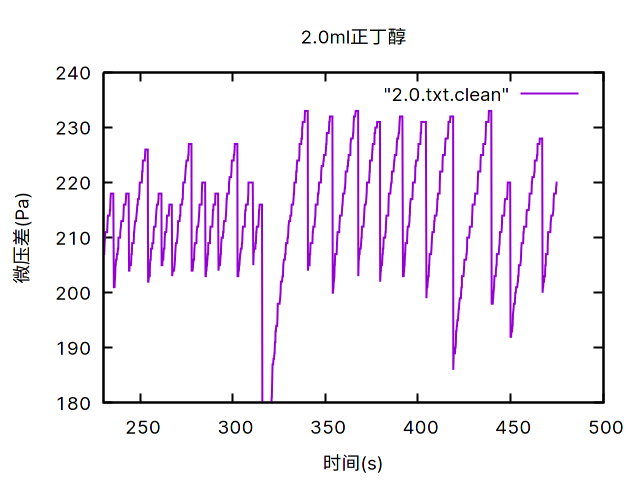
\includegraphics[width=.9\linewidth]{../img/2.0.png}
\end{center}

最大压强差读数数据记录如下:
\begin{center}
\begin{tabular}{lrrrrrrr}
序号 & 1 & 2 & 3 & 4 & 5 & 6 & 平均\\
\hline
最大压强差读数\(\Delta\) p(Pa) & 233 & 232 & 233 & 231 & 232 & 231 & 232\\
\end{tabular}
\end{center}

最大压强读数平均:
\[
    \Delta p =\frac{233+233+232+232+231+231}{6}=232(Pa)
    \]
由公式 \(\sigma\)=K\(\cdot\) \(\Delta\) p 可得表面张力为:
\[
    \sigma=K\cdot \Delta p=2.2703\times 10^{-4}\times 232=52.67\times 10^{-3}(N\cdot m^{-1})
    \]

\section{2.4mL 正丁醇}
\label{sec:org05c7c87}
    100 mL 容量瓶中含 2.4 mL 正丁醇。由于正丁醇分子量为 74.14,密度为 0.8109 g/cm\textsuperscript{3}
故得正丁醇浓度为:2.4\texttimes{} 0.8109/(74.14\texttimes{} 0.1)=0.26250 mol/L=262.50 mol/m\textsuperscript{3}.

电脑记录数据作图如下:
\begin{center}
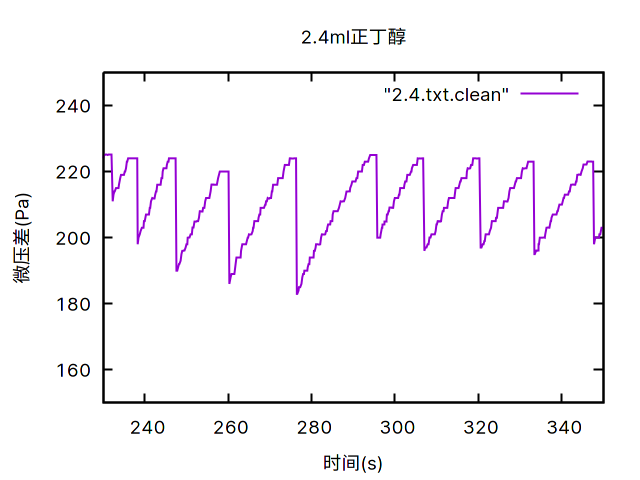
\includegraphics[width=.9\linewidth]{../img/2.4.png}
\end{center}

最大压强差读数数据记录如下:
\begin{center}
\begin{tabular}{lrrrrrrr}
序号 & 1 & 2 & 3 & 4 & 5 & 6 & 平均\\
\hline
最大压强差读数\(\Delta\) p(Pa) & 224 & 225 & 224 & 224 & 223 & 223 & 224\\
\end{tabular}
\end{center}

最大压强读数平均:
\[
    \Delta p =\frac{224\times 3+223\times 2+225}{6}=224(Pa)
    \]
由公式 \(\sigma\)=K\(\cdot\) \(\Delta\) p 可得表面张力为:
\[
    \sigma=K\cdot \Delta p=2.2703\times 10^{-4}\times 224=50.85\times 10^{-3}(N\cdot m^{-1})
    \]

\section{2.8mL 正丁醇}
\label{sec:org8b35d89}
    100 mL 容量瓶中含 2.8 mL 正丁醇。由于正丁醇分子量为 74.14,密度为 0.8109 g/cm\textsuperscript{3}
故得正丁醇浓度为:2.8\texttimes{} 0.8109/(74.14\texttimes{} 0.1)=0.30625 mol/L=306.25 mol/m\textsuperscript{3}.

电脑记录数据作图如下:
\begin{center}
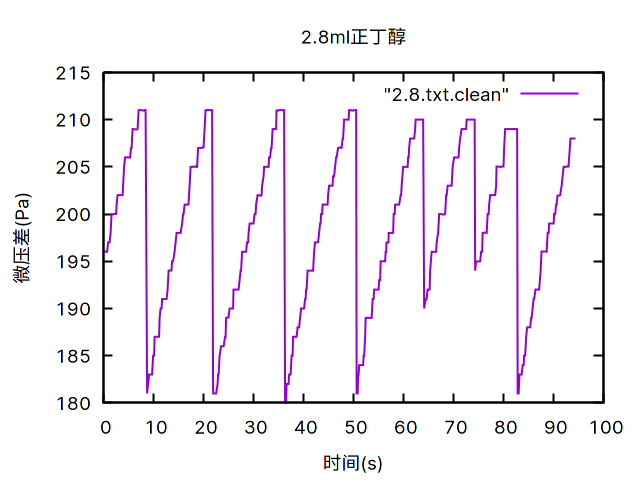
\includegraphics[width=.9\linewidth]{../img/2.8.png}
\end{center}

最大压强差读数数据记录如下:
\begin{center}
\begin{tabular}{lrrrrrrr}
序号 & 1 & 2 & 3 & 4 & 5 & 6 & 平均\\
\hline
最大压强差读数\(\Delta\) p(Pa) & 211 & 211 & 211 & 211 & 210 & 210 & 211\\
\end{tabular}
\end{center}

最大压强读数平均:
\[
    \Delta p =\frac{211\times 4+210\times 2}{6}=211(Pa)
    \]
由公式 \(\sigma\)=K\(\cdot\) \(\Delta\) p 可得表面张力为:
\[
    \sigma=K\cdot \Delta p=2.2703\times 10^{-4}\times 211=47.90\times 10^{-3}(N\cdot m^{-1})
    \]

\chapter{作表面张力与浓度(\(\sigma\)-c)的关系图,求吸附量\(\Gamma\)}
\label{sec:org39f37c0}

作\(\sigma\)-c图,用多次方拟合各个数据点,得到光滑曲线和曲线的多项式方程\(\sigma\) =f(c);
微商后得到切线微分方程式
\[
   \frac{d\sigma}{dc}=f'(c)
   \]
如下图所示。在光滑曲线上选取 6-7 个浓度点,代入
\[
   \Gamma=-\frac{c}{RT}\left(\frac{d\sigma}{dc}\right)
   \]
计算不同浓度溶液的吸附量\(\Gamma\) 值.

\begin{center}
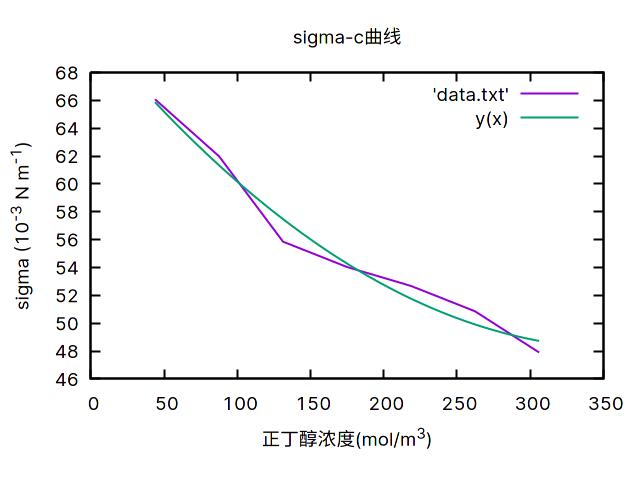
\includegraphics[width=.9\linewidth]{../img/sigma-1.png}
\end{center}
其中
\[
   y=ax^{2}+bx+c
   \]
\begin{itemize}
\item a = 0.000175207
\item b = -0.126588
\item c = 71.0671
\end{itemize}

\begin{verbatim}
correlation matrix of the fit parameters:
.	a      	b      	c      
a	1.000 
b	-0.977  1.000 
c	0.840 	-0.924	1.000 
\end{verbatim}

进行二次多项式拟合所得方程为:
\[
	\sigma=1.75207\times 10^{-4}C^{2}-0.126588C+71.0671
	\]
微商后得切线微分方程式
\[
	\frac{d\sigma}{dc}=3.50414\times 10^{-4}C-0.126588
	\]
\section{C\textsubscript{1}}
\label{sec:org8ef1cb9}
\[
    \Gamma_{1}=-\frac{43.75}{8.314\times 298.15}\times (3.50414\times 10^{-7}\times 43.75-0.126588\times 10^{-3})=1.963641\times 10^{-6} mol/m^{2}
    \]
\[
    \frac{C}{\Gamma}=2.218837\times 10^{7}m^{-1}
    \]

\section{C\textsubscript{2}}
\label{sec:org4ff173c}
\[
    \Gamma_{2}=-\frac{87.50}{8.314\times 298.15}\times (3.50414\times 10^{-7}\times 87.50-0.126588\times 10^{-3})=3.386126\times 10^{-6} mol/m^{2}
    \]
\[
    \frac{C}{\Gamma}=2.584074\times 10^{7}m^{-1}
    \]

\section{C\textsubscript{3}}
\label{sec:org414ab70}
\[
    \Gamma_{3}=-\frac{131.25}{8.314\times 298.15}\times (3.50414\times 10^{-7}\times 131.25-0.126588\times 10^{-3})=4.267454\times 10^{-6} mol/m^{2}
    \]
\[
    \frac{C}{\Gamma}=3.075604\times 10^{7}m^{-1}
    \]
\section{C\textsubscript{4}}
\label{sec:orgb600c8a}
\[
    \Gamma_{4}=-\frac{175.00}{8.314\times 298.15}\times (3.50414\times 10^{-7}\times 175.00-0.126588\times 10^{-3})=4.607626\times 10^{-6} mol/m^{2}
    \]
\[
    \frac{C}{\Gamma}=3.798051\times 10^{7}m^{-1}
    \]

\section{C\textsubscript{5}}
\label{sec:org2ab4d01}
\[
    \Gamma_{5}=-\frac{218.75}{8.314\times 298.15}\times (3.50414\times 10^{-7}\times 218.75-0.126588\times 10^{-3})=4.406642\times 10^{-6} mol/m^{2}
    \]
\[
    \frac{C}{\Gamma}=4.964098\times 10^{7}m^{-1}
    \]


\section{C\textsubscript{6}}
\label{sec:orgafdef19}
\[
    \Gamma_{6}=-\frac{262.50}{8.314\times 298.15}\times (3.50414\times 10^{-7}\times 262.50-0.126588\times 10^{-3})=3.664501\times 10^{-6} mol/m^{2}
    \]
\[
    \frac{C}{\Gamma}=7.163321\times 10^{7}m^{-1}
    \]

\chapter{作图求饱和吸附量\(\Gamma\)\textsubscript{\(\infty\)}}
\label{sec:orgb5af31f}

由直线斜率根据公式
\[
   \frac{C}{\Gamma}=\frac{C}{\Gamma_{\infty}}+\frac{1}{K\Gamma_{\infty}}
   \]
\begin{center}
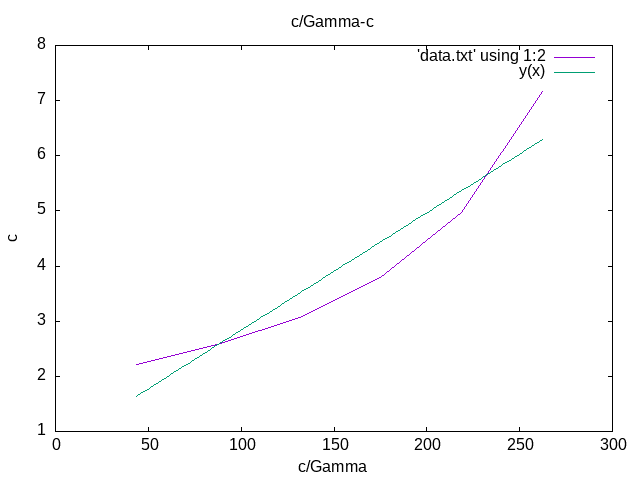
\includegraphics[width=.9\linewidth]{../img/out.png}
\end{center}


\begin{itemize}
\item k               = 0.02128          +/- 0.0037       (17.39\%)
\item b               = 0.708837         +/- 0.6304       (88.93\%)

则
\[
   \Gamma_{\infty}=\frac{1}{k}=4.699248\times 10^{-6} mol/m^{3}
   \]
正丁醇分子的横截面积为:
\[
   S_{0}=\frac{1}{\Gamma_{\infty}\widetilde{N}}=3.533627\times 10^{-19} m^{2}
   \]
\end{itemize}
\end{document}
